%! TeX program = lualatex
\documentclass[../main.tex]{subfiles}
\begin{document} \section{Review of piecewise functions and absolute values}
The left-brace notation for a piecewise function \(f(x)\) prescribes expressions for \(f(x)\) on two or more \emph{non-intersecting} intervals called subdomains. Each line in the left-brace notation is the expression for \(f(x)\) on the specified subdomain.  The domain for \(f(x)\) is the union of all its subdomains.

\blanklines{10}

\begin{mdframed}[style=simple-compact]
  \faExclamationTriangle{} One-sided limits are \hlmain{universal fail-safe tools} to solve calculus problems (evaluate \hlsupp{limits}, classify \hlsupp{discontinuities}, calculate \hlsupp{derivatives}, etc) \hlwarn{at endpoints of subdomains} of piecewise functions.  The specific expression in the limit is \emph{not always} just \(f(x)\) and depends on the problem.
\end{mdframed}

\begin{exercise}
  Sketch the function
  \(
  f(x) = 
  \begin{cases}
    x + 1, &x > 2 \\
    2, &x \le 1
  \end{cases}
  \).

  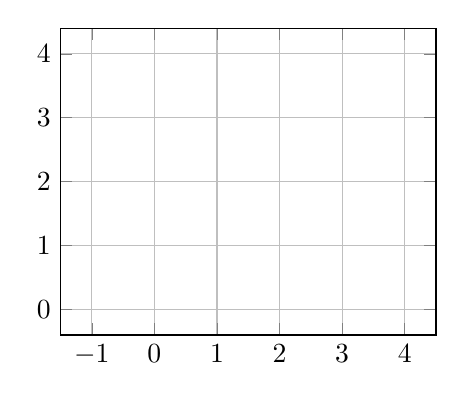
\begin{tikzpicture}
    \begin{axis}[xmin=-1, xmax=4, ymin=0, ymax=4, grid=major, width=2.5in, xtick={-1,0,...,4}, ytick={0,1,...,4}, enlargelimits=true]
    \end{axis}
  \end{tikzpicture}
\end{exercise}

\begin{exercise}
  The graph of a function \(g(x)\) on domain \([-2,5]\) is given below. Express \(g(x)\) using the left-brace notation.

  \begin{minipage}{3in}
    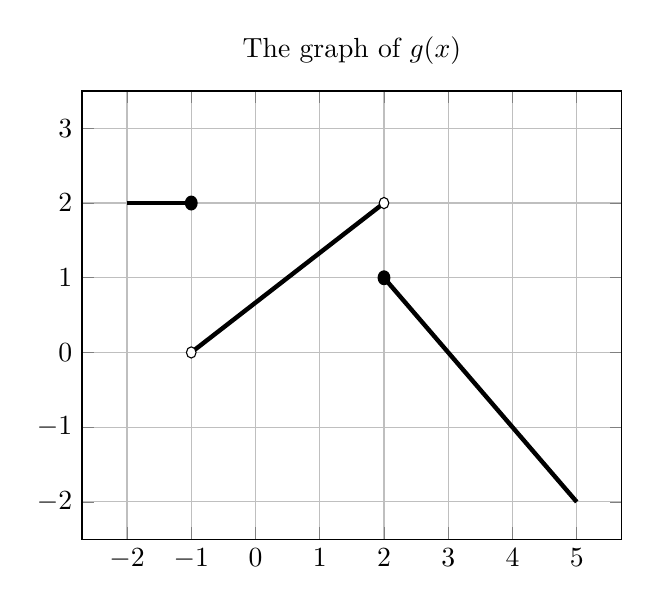
\begin{tikzpicture}
      \begin{axis}[
        enlargelimits=true,
        xmin=-2, xmax=5,
        ymin=-2, ymax=3,
        xtick={-2,-1,...,5},
        ytick={-2,-1,...,3},
        grid=major,
        title={The graph of \(g(x)\)},
        ]
        \addplot[ultra thick] coordinates {(-2, 2) (-1, 2)};
        \addplot[ultra thick] coordinates {(-1, 0) ( 2, 2)};
        \addplot[ultra thick] coordinates {( 2, 1) ( 5,-2)};
        \fill (axis cs:-1,2) circle[radius=0.1];
        \fill (axis cs: 2,1) circle[radius=0.1];
        \draw[fill=white] (axis cs:-1,0) circle (0.075);
        \draw[fill=white] (axis cs:2,2) circle (0.075);
      \end{axis}
    \end{tikzpicture}
  \end{minipage}
  \begin{minipage}{2in}
    \[
      g(x) = 
      \begin{cases}
        \phantom{a} \\[10ex]
        \phantom{a}
      \end{cases}
    \]
  \end{minipage}
\end{exercise}

\clearpage

We now review absolute values. The absolute value function is fundamentally a piecewise function.
\begin{equation} \label{eq:abs}
  |x| = 
  \begin{cases}
    x, &\text{if } x \ge 0, \\
    -x, &\text{if } x < 0.
  \end{cases}
\end{equation}

\faExclamationTriangle{} The expression \(|x| = \sqrt{x^{2}}\) \hlwarn{hides details}, encourages silly algebraic mistakes, and \hlwarn{makes easy-to-miss details even harder to be noticed}.  You are \hlmain{strongly advised} to always use Equation~\eqref{eq:abs}.  

For the purpose of making sense of absolute value of functions, please remember that the input \(x\) shows up in five different places in Equation~\eqref{eq:abs}.  

\blanklines{5}

Exercise~\ref{ex:piecewise-abs-of-function} is \hlmain{a fail-safe starting step} to solve problems like \enquote{Find all numbers at which \(\left| \frac{x + 2}{x - 4} \right|\) is blah blah \dots.}

\begin{exercise} \label{ex:piecewise-abs-of-function}
  Understand \(|(x + 2)(x - 4)|\) and \(\left| \frac{x + 2}{x - 4} \right|\) as piecewise functions.

  \blanklines{35}
\end{exercise}
\end{document}
